%%%%%%%%%%%%%%%%%%%%%%%%%%%%%%%%
% Chap 3. PPO Lagrangian Network
%%%%%%%%%%%%%%%%%%%%%%%%%%%%%%%%

\chapter{PPO-based Method in State-wise Constrained RL}\label{chapter3}

\section{PPO Lagrangian Network}

As discussed in Section ~\ref{chap2:sec5:fac}, Feasible Actor-Critic (FAC) exhibits potential limitations arising from the characteristics of the SAC algorithm, its off-policy nature, and the way state-wise safety is defined through the cost Q-function.
In this chapter, we introduce our proposed method, which extends PPO under the state-wise constrained RL framework.
Similar to FAC method, we employ a network that estimates state-wise Lagrange multipliers to enforce safety constraints at the state level.
Thus, objective function of the policy is modified to include a Lagrange multiplier network:
% \begin{equation} \label{chap3:eq:ppo_lagnet}
%   J^{\text{PPO-Lagnet}}(\theta) = \mathbb{E}_{\pi_{\theta_\text{old}}} \left[ \min \left( r(\theta) A^{\pi_{\theta_\text{old}}}(s, a), \text{clip}(r(\theta), 1 - \epsilon, 1 + \epsilon)A^{\pi_{\theta_\text{old}}}(s, a) \right) - \lambda_\xi(s) r(\theta) A^{\pi_{\theta_\text{old}}}_c \right]
% \end{equation}
\begin{equation} \label{chap3:eq:ppo_lagnet}
  \begin{aligned}
    J^{\text{PPO-Lagnet}}(\theta) = \mathbb{E}_{\pi_{\theta_\text{old}}} \Big[ &\min \big( r(\theta) A^{\pi_{\theta_\text{old}}}(s, a), \text{clip}(r(\theta), 1 - \epsilon, 1 + \epsilon) A^{\pi_{\theta_\text{old}}}(s, a) \big) \\
    &- \lambda_\xi(s) r(\theta) A^{\pi_{\theta_\text{old}}}_c \Big]
  \end{aligned}
\end{equation}
where $A^{\pi_{\theta_\text{old}}}_c$ is the advantage function for the cost and $\lambda_\xi(s)$ is the Lagrange multiplier network that estimates the Lagrange multiplier for the cost at state $s$.
The Lagrange multiplier network is iteratively updated during training to guide the policy toward satisfying the imposed constraints.
The update of the Lagrange multiplier network depends on whether the empirical cost at state $s$ exceeds the threshold $w$:
\begin{equation}
  \lambda(s) \leftarrow \lambda(s) + \beta(\hat{J}_c - w)
\end{equation}
To ensure the positivity of the Lagrange multiplier, a softplus activation function is applied to the final layer of the network. 
\begin{figure*}[h]
  \centering
  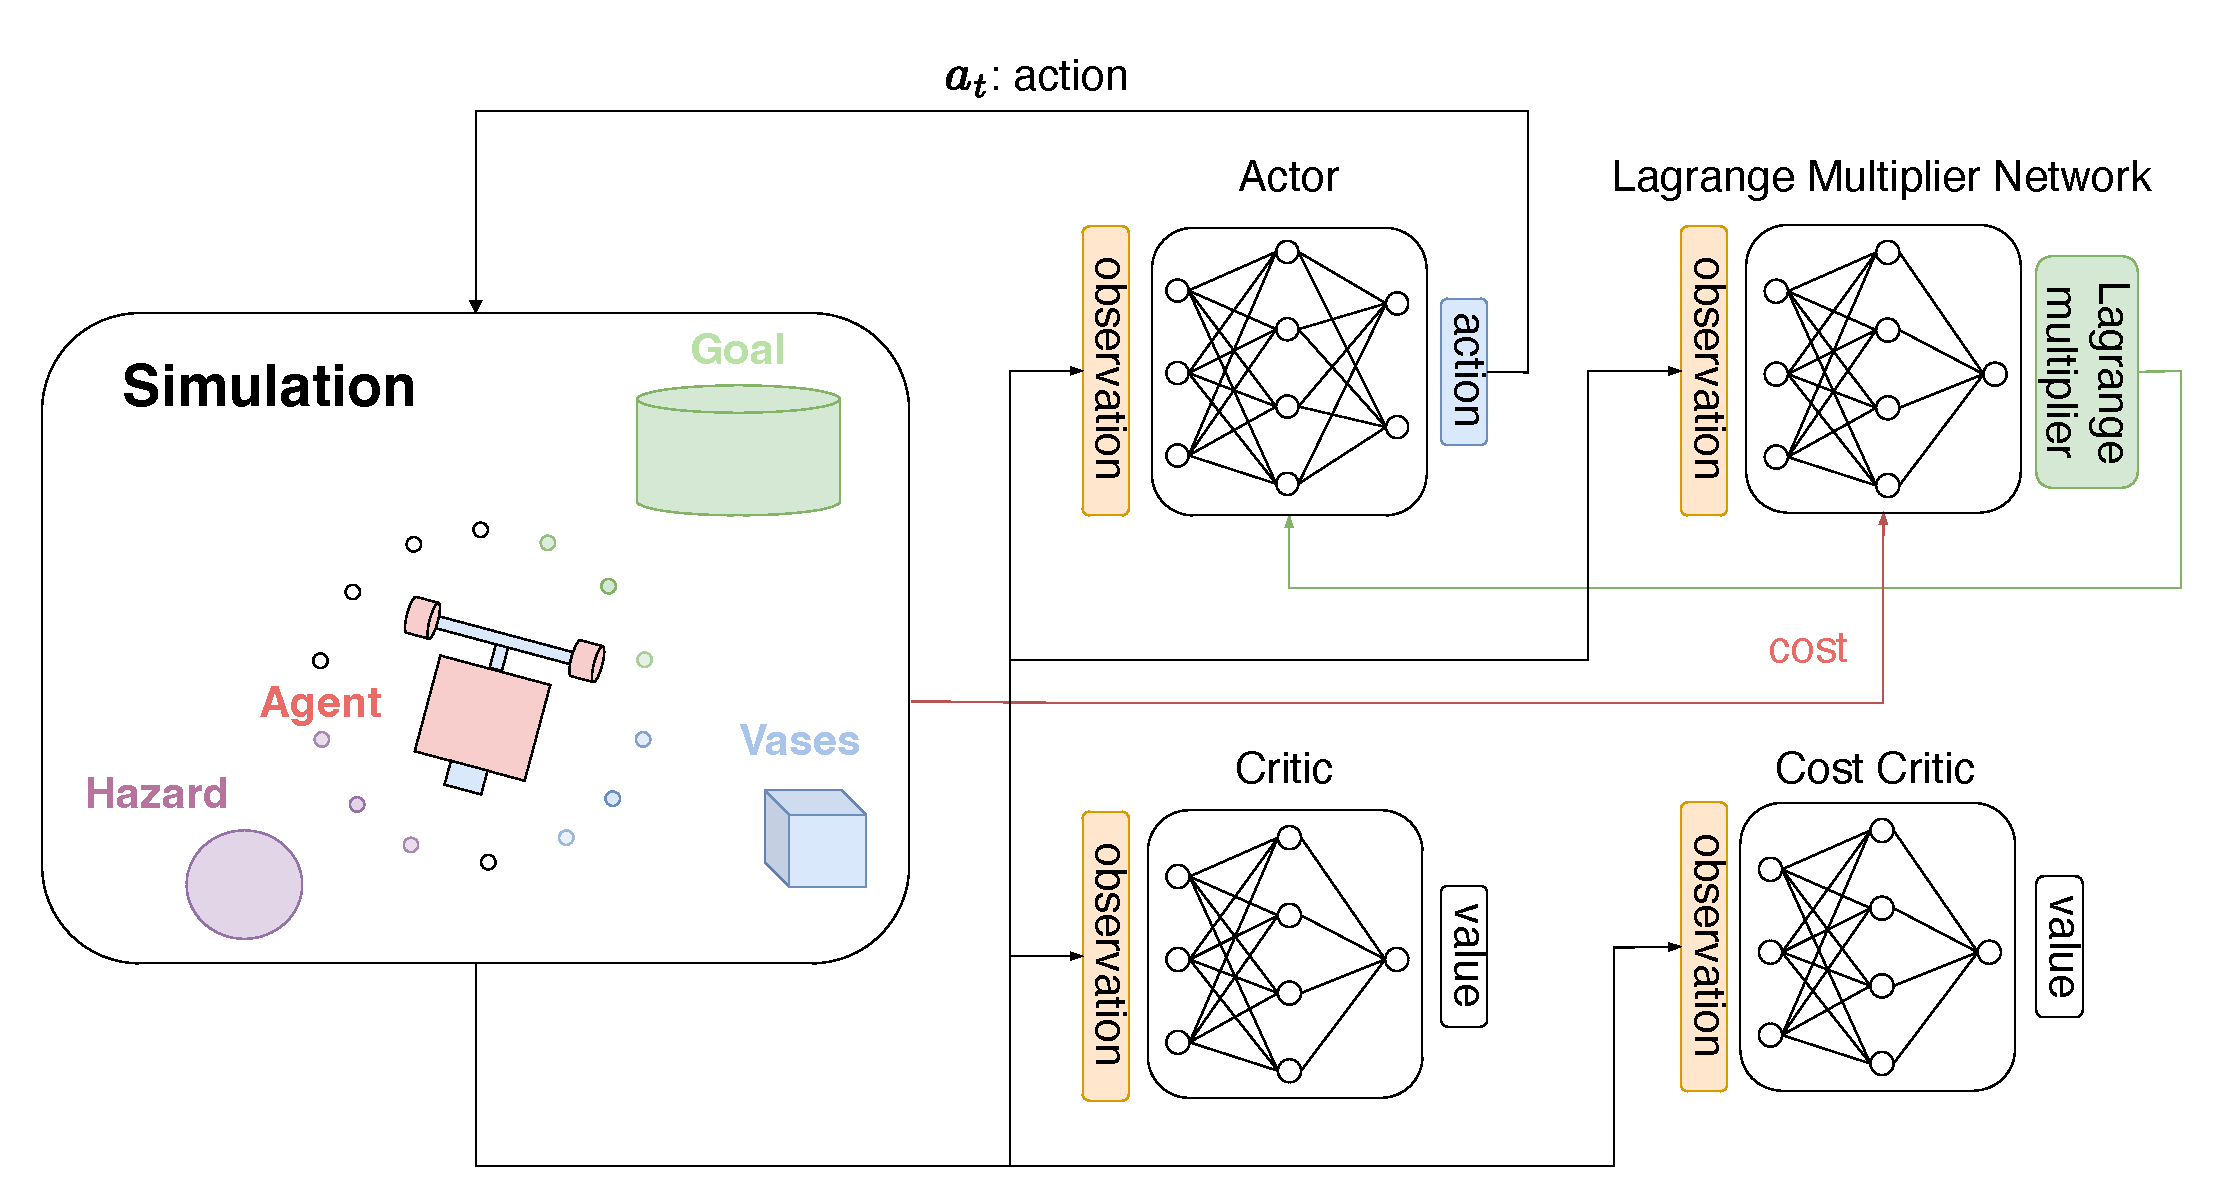
\includegraphics[width=1.0\textwidth]{imgs/chap3/ppo_lagnet.pdf}
  \caption{Structure of PPO Lagrangian Network}
  \label{chap3:fig:ppo_lagnet}
\end{figure*} \\
The overall architecture of the PPO Lagrangian Network is illustrated in Fig.~\ref{chap3:fig:ppo_lagnet}. 
The structure closely follows that of PPO Lagrangian described in Fig.~\ref{chap2:fig:ppo_lag}: 
the agent interacts with the environment using actions generated by the actor network, and the collected trajectories are used to estimate reward and cost returns at each state using the value function networks.
These return estimates are then used to compute the reward and cost advantages, which correspond to $A^{\pi_{\theta_\text{old}}}$ and $A^{\pi_{\theta_\text{old}}}_c$.
These advantages are then used to update the policy according to Equation~\ref{chap3:eq:ppo_lagnet}.
The key distinction from the PPO Lagrangian lies in the design of the Lagrange multiplier. 
Instead of using a single scalar multiplier, the PPO Lagrangian Network introduces a dedicated neural network that estimates a state-wise Lagrange multiplier $\lambda_\xi(s)$, which is updated based on the cost incurred at each individual state within the trajectories.
This allows the algorithm to enforce constraints more precisely at the state level rather than relying on trajectory-level cost.

\begin{algorithm}
  \DontPrintSemicolon
  \caption{PPO Lagrangian Network}
  \KwIn{Initial policy parameters $\theta_0$, initial value function parameters $\phi_0$, initial cost value function parameters $\phi^c_0$, Lagrange multiplier network parameters $\xi$, threshold $w$}
  \For{each epoch $k = 0, 1, 2, \cdots$}{
    \For{each time step $t = 1$ \KwTo $T$}{
      \tcp{Collect trajectories}
      Sample action $a_t \sim \pi_{\theta_{t - 1}}(s_t)$ \;
      Execute action $a_t$ in the environment and observe reward $r_t$, cost $c_t$ and next state $s_{t + 1}$ \;
      Store transition $\tau_t = (s_t, a_t, r_t, c_t, s_{t+1})$ in buffer $D_k$ \;

      \If{episode end}{
        Compute rewards-to-go $\hat{R}_t$ and advantage estimates $\hat{A}_t$ based on the current value function $V_{\phi_k}$ \;
        Compute costs-to-go $\hat{R}^c_t$ and cost advantage estimates $\hat{A}^c_t$ based on the current cost value function $V^c_{\phi_k}$ \;
      }
    }
    \BlankLine
    
    \tcp{Lagrange multiplier network update}
    Update the Lagrange multiplier $\lambda$ by gradient ascent:
    \begin{equation*}
        \xi_{k + 1} = \xi_k + \beta \left[ \frac{1}{|D_k|T} \sum_{\tau \in D_k} \sum^T_{t = 0} (c_t - w) \right]
    \end{equation*}
    \BlankLine

    \tcp{Policy update}
    Update the policy parameters $\theta$ by maximizing the objective function:
    \begin{equation*}
      \begin{aligned}
        \theta_{k + 1} = \arg \max_\theta \frac{1}{|D_k|T} \sum_{\tau \in D_k} \sum^T_{t = 0} \Big[ &\min \left( r_t(\theta) \hat{A}^{\pi_{\theta_k}}(s_t, a_t), \; g\left( \epsilon, \hat{A}^{\pi_{\theta_k}}(s_t, a_t) \right) \right) \\
        & - \lambda_\xi (s_t) r_t(\theta) \hat{A}^{\pi_{\theta_k}}_c (s_t, a_t)  \Big]\\
        \text{where }
        r_t(\theta) = \frac{\pi_\theta(a_t|s_t)}{\pi_{\theta_k}(a_t|s_t)}, \;
        &g(\epsilon, A) = 
          \begin{cases}
            (1 + \epsilon)A \quad A \geq 0 \\
            (1 - \epsilon)A \quad A < 0
          \end{cases}
      \end{aligned}
    \end{equation*}    
    \BlankLine

    \tcp{Value function update}
    Fit value function by regression on mean-squared error:
    \begin{equation*}
      \begin{aligned}
        \phi_{k + 1} &= \arg\min_\phi \frac{1}{|D_k|T} \sum_{\tau \in D_k} \sum^T_{t = 0} \left( V_\phi(s_t) - \hat{R}_t \right)^2 \\
        \phi^c_{k + 1} &= \arg\min_\phi \frac{1}{|D_k|T} \sum_{\tau \in D_k} \sum^T_{t = 0} \left( V_{\phi^c}(s_t) - \hat{R}^c_t \right)^2
      \end{aligned}
    \end{equation*}
    % typically via stochastic gradient descent algorithm.
  }
\end{algorithm}

\subsection{Comparison with PPO Lagrangian}

In PPO Lagrangian, the Lagrange multiplier is a scalar because it enforces that the cumulative cost along trajectories generated by the policy $\pi_\theta$ remains below a specified threshold.
In contrast, PPO Lagrangian Network estimates a state-wise Lagrange multiplier, which enables the policy to satisfy cost constraints more precisely at each individual state by enforcing the cost at each state to remain below the specified threshold.

\subsection{Comparison with Feasible Actor-Critic}

Feasible Actor-Critic (FAC) is similar to PPO Lagrangian Network in that it also estimates a state-wise Lagrange multiplier.
However, unlike FAC, our method updates the Lagrange multiplier network in a different way.
In FAC, the update is based on the output of the cost action-value network, which estimates the state-wise cost value.
In contrast, our proposed method updates the policy based on the actual cost values observed for each state.